\documentclass{beamer}
\usetheme{Boadilla}

\usepackage{amsmath}
\usepackage{amsfonts}
\usepackage{hyperref}

\usepackage{amsmath}
\DeclareMathOperator*{\argmax}{arg\,max}
\DeclareMathOperator*{\argmin}{arg\,min}

\title{Black-box $\alpha$-divergence minimization}
\author{Galina Boeva}
\institute{MIPT, 2023}


\begin{document}

\begin{frame}
    \titlepage
\end{frame}


\begin{frame}
    \tableofcontents
\end{frame}


\section{Motivation}
\begin{frame}{Motivation}
    \begin{block}{Main idea}
    This is a general method for approximating $\alpha$ - divergence, which combines approaches such as variational Bayes and expectation propagation.
    \end{block} 
\end{frame}

\section{Definition}
\begin{frame}{Definition}
    \begin{block}{Posterior distribution}
    \begin{equation}
        p(\theta | \mathcal{D}) \propto \left[\displaystyle\prod_{n=1}^N p(x_n|\theta)\right] p_0(\theta),
    \end{equation} 
        where $p(x_n|\theta)$ is a likelihood factor and $p_0(\theta)$ is the prior.
    \end{block}
    \begin{block}{$\alpha$-divergence}
    \begin{equation}
        D_{\alpha}[p||q] = \frac{1}{\alpha(1 − \alpha)}\left(1 - \int p(\theta)^{\alpha} q(\theta)^{1−\alpha}d\theta\right)
    \end{equation} 
    \[D_1[p||q] = \lim_{\alpha\to1} D_{\alpha}[p||q] = KL[p||q]\]
    \[D_0[p||q] = \lim_{\alpha\to0} D_{\alpha}[p||q] = KL[q||p]\] 
    \end{block}
\end{frame}

\begin{frame}{Definition}
    
     \begin{figure}
        \centering
        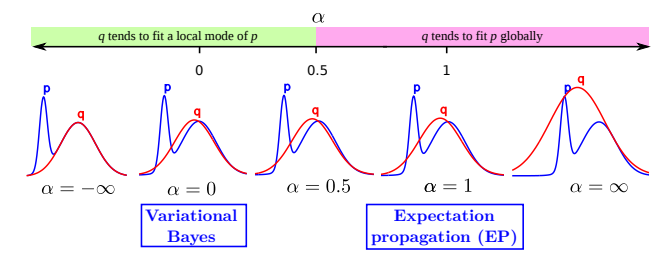
\includegraphics[scale=0.7]{images/div_alpha.png}
        \caption{An illustration of approximating distributions by $\alpha$-divergence minimization. Here p and q shown in the graphs are unnormalized probability densities.}
        \label{fig:enter-label}
    \end{figure}
    
\end{frame}


\section{Methods}
\begin{frame}{Approximate local minimization of
$\alpha$-divergences}
\centering
\begin{block}{Power EP energy}

\begin{equation}
\begin{split}
    E(\lambda_0, {\lambda_n}) = \log Z(\lambda_0) + \left(\frac{N}{\alpha} - 1\right) \log Z(\lambda_q) 
    \\- \frac{1}{\alpha} \sum_{n=1}^N \log \int Z p(x_n|\theta)^{\alpha} \exp\{s(\theta)^T (\lambda_q - \alpha \lambda_n)\} d\theta
\end{split}
\end{equation}
where 

1. $p_0(\theta) = \exp\{s(\theta)^T \lambda_0 - \log Z(\lambda_0)\} $,

2. $f_n(\theta) = \exp\{s(\theta)^T \lambda_n\}$, 

3. $q(\theta) \propto \exp\{s(\theta)^T (\sum_{n}\lambda_n + \lambda_0)\}$, 

4. $\lambda_q = \sum_n \lambda_n + \lambda_0$ .
    \end{block}
 
\end{frame}

\begin{frame}{Approximate local minimization of
$\alpha$-divergences}
\centering
\begin{figure}
        \centering
        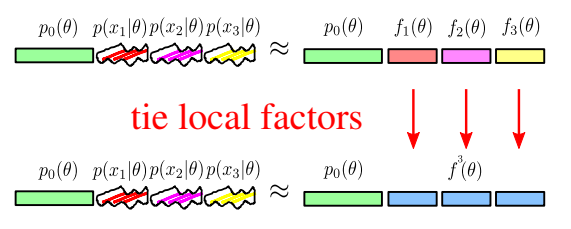
\includegraphics[scale=0.62]{images/div_bmm_6.png}
        \caption{A cartoon for BB-$\alpha$’s factor tying constraint. Here we assume the dataset has N = 3 observations. }
        \label{fig:enter-label}
    \end{figure}
 
\end{frame}

\begin{frame}{Approximate local minimization of
$\alpha$-divergences}
\centering
\begin{block}{Power EP energy}
Let all the site parameters to be equal, i.e. $\lambda_n = \lambda$ $\forall n$. Thus, $f_n(\theta) = f(\theta)$ $\forall n$ . The cavity distributions with natural parameter:$$ \lambda^{\n} = (N - \alpha)\lambda + \lambda_0, \lambda_q = N\lambda + \lambda_0$$ 

Thus, rewrite (3):

\begin{equation}
\begin{split}
    E(\lambda_0,\lambda) = \log Z(\lambda_0) - \log Z(\lambda_q) - 
    \\ - \frac{1}{\alpha} \sum_{n=1}^N \log E_q \left(\left(\frac{p(x_n|\theta)}{f(\theta)}\right)^{\alpha}\right)
\end{split}
\end{equation}
\end{block}
 
\end{frame}


\section{Empirical results}
\begin{frame}{Empirical results}
    \begin{figure}
        \centering
        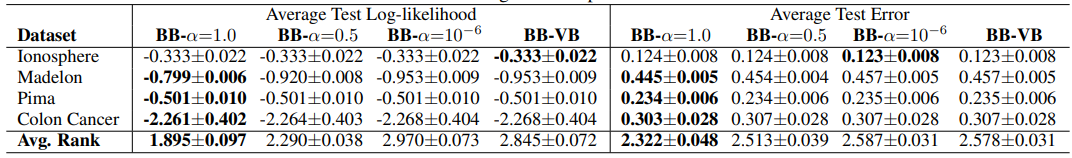
\includegraphics[scale=0.62]{images/div_bmm_3.png}
        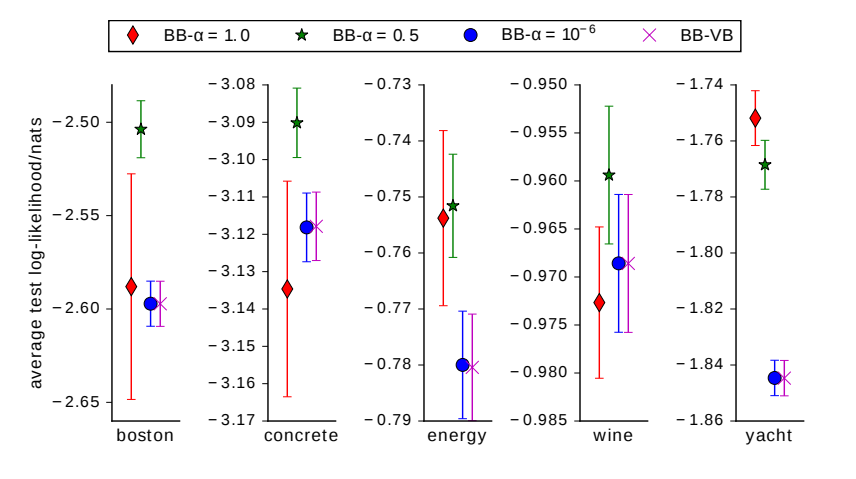
\includegraphics[scale=0.5]{images/div_bmm_4.png}
        \caption{1. Probit regression experiment results 
        2. Average test log-likelihood and the ranking comparisons.}
        \label{fig:enter-label}
    \end{figure}
\end{frame}

\begin{frame}{Empirical results}
    \begin{figure}
        \centering
        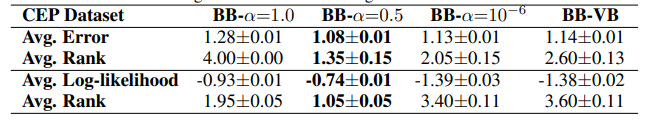
\includegraphics[scale=0.7]{images/div_bmm_5.png}
        \caption{Average Test Error and Test Log-likelihood in CEP Dataset.}
        \label{fig:enter-label}
    \end{figure}
\end{frame}


\begin{frame}{Literature}
    \begin{enumerate}
        \item \textbf{Main article} \href{http://proceedings.mlr.press/v48/hernandez-lobatob16.pdf}
        {Black-Box $\alpha$-Divergence Minimization}.
    \end{enumerate}
\end{frame}



\end{document}